\documentclass[a4paper, oneside]{discothesis}

\usepackage[utf8]{inputenc}
\usepackage[T1]{fontenc}
\usepackage{minted}
\usepackage{subcaption}

%%%%%%%%%%%%%%%%%%%%%%%%%%%%%%%%%%%%%%%%%%%%%%%%%%%%%%%%%%%%%%%%%%%%%%%%%%%%%%%%%%%%%%%%%%%%%%%%%
% DOCUMENT METADATA

\thesistype{Semester Thesis} % Master's Thesis, Bachelor's Thesis, Semester Thesis, Group Project
\title{End to End Encryption in a Cloud-Based Messenger}

\author{Noah Zarro}
\email{zarron@ethz.ch}

\institute{Distributed Computing Group \\[2pt]
Computer Engineering and Networks Laboratory \\[2pt]
ETH Zürich}

% Optionally, you can put in your own logo here
\logo{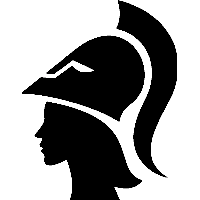
\includegraphics[width=0.2\columnwidth]{figures/logo_black.png}}

\supervisors{Ard Kastrati, Karolis Martinkus\\[2pt] Prof.\ Dr.\ Roger Wattenhofer}

% Optionally, keywords and categories of the work can be shown (on the Abstract page)
%\keywords{Keywords go here.}
%\categories{ACM categories go here.}

\date{\today}

%%%%%%%%%%%%%%%%%%%%%%%%%%%%%%%%%%%%%%%%%%%%%%%%%%%%%%%%%%%%%%%%%%%%%%%%%%%%%%%%%%%%%%%%%%%%%%%%%

\begin{document}

\frontmatter % do not remove this line
\maketitle

\cleardoublepage

\begin{abstract}

In the time of rising public awareness for the privacy of messenger apps, people start using Telegram or Signal, instead of WhatsApp. But since Telegram does not offer end-to-end encryption, and Signal does not offer cloud functionality, there is no ideal choice that unifies both features. This paper aims to change this, and proposes a generic end-to-end encryption overlay for cloud-based messengers such as Telegram, or even Facebook Messenger.

\end{abstract}

\tableofcontents

\mainmatter % do not remove this line

% Start writing here

\chapter{Motivation}
On the 7th of January 2021, Elon Musk tweeted the following two words: "Use Signal!" \cite{Twitter}. It was a tweet with lots of consequences. First, it caused the stock prices of the totally unrelated company \emph{Signal Advance} to skyrocket. Secondly, and more relevant for this paper, it once again fueled the discussion about messengers. The tweet was a reaction to the announcement of WhatsApp's new terms and conditions, that once again weakened the privacy of its users. Soon after, WhatsApp's competitors were able to report rapid increases of their number of users.

But there are immense differences among the other players in the market of messengers. It is worth a closer look, see Table \ref{table:messengers}. When switching from WhatsApp to another app, there are two reasonable options: Either Telegram, that offers cloud functionality, which means if one loses his phone, previously sent messages are preserved. But it does not offer end-to-end (E2E) encryption, except for unhandy peer to peer, device locked chats, which are not cloud-based. However, it provides by far the most features, such as bots, custom clients, GIFs, etc. On the other hand, Signal is considered the most secure messenger of the four in question, since it provides forward secrecy, automatic \emph{healing} after one round trip if keys were leaked, groups members that are anonymous to the server, etc. Threema however does neither offer forward secrecy, nor cloud, and it is not free of charge, so there is no real unique selling point to it.

But if one wants to have a cloud-based messenger that is also E2E-encrypted, there is currently no option. This thesis aims to solve this problem, by presenting an app that provides both features. But since there are already that many messengers, there is no need to develop a new messenger from scratch. Therefore, an app is presented that acts as a client for multiple existing cloud-based messengers services and adds an E2E-encryption layer to them. For now, the client only supports Telegram, but additional messengers, like Facebook, could be easily added.


\begin{table}[h!]
\centering
\begin{center}
 \begin{tabular}{|| c ||c c c c||} 
  \hline
 \multicolumn{5}{|c|}{Popular Messengers} \\
 \hline
 \hline
   & WhatsApp & Telegram & Threema & Signal \\ [0.5ex] 
 \hline\hline
 Users (M) & 2'000 & 500 & 10 & 40 \\ 
 \hline
 E2E-Encryption & claimed\footnotemark & no & yes & yes \\
 \hline
 Forward Secrecy & claimed\footnotemark[\value{footnote}] & no & no & yes \\
 \hline
 Cloud & backup & yes & no & no \\
 \hline
 Open Source & no & yes (client) & yes & yes \\
 \hline
\end{tabular}
\end{center}
\caption{Comparison of Messengers, numbers taken from \cite{Business, Statistia}}
\label{table:messengers}
\end{table}

\footnotetext{WhatsApp is not open source, so it cannot be checked}

\chapter{Protocol}

\section{Overview}
The goal of the system is to provide an E2E-encryption overlay for a generic cloud-based messenger, like Telegram or Facebook Messenger. There are several desired properties the overlay should have.

\begin{enumerate}
  \item A user should be able to log in from different devices with the same account and see all previously sent messages. 
  \item The cloud infrastructure of the underlying messenger should be used for messages.
  \item Peer to peer chats and group chats should be E2E-encrypted.
\end{enumerate}

In the following, the details of the concept are elaborated. First, it is explained how the cloud feature is achieved. In the next part, the basic peer to peer encryption is introduced, and the final part covers the encryption of group chats.

\section{Cloud}

Since an existing, cloud-based messenger should be used, all messages must be saved on its server. In the implementation, Telegram was used as a base messenger. Therefore, the protocol needs a custom client, that can encrypt and decrypt messages and exchange them with the server. So far it resembles a generic end-to-end encrypted messenger, as there are many on the market, like WhatsApp, Signal and Threema. But since the underlying messenger is cloud-based, the client should be able to log in from multiple devices and see the same messages. This is the main problem of this thesis, and the two most promising solutions are elaborated in the following.

\subsection{Mulitple Keys}

One approach, which Signal followed in the Sesame protocol \cite{Sesame}, is to create an artificial "group" chat with all devices of a user and its peer as members, in which a message is sent to each member individually. In this approach, each device has a unique key, and if a message is sent from one device, it is encrypted once for each other device in the "group". These messages are then sent to the corresponding devices and stored locally. The problem with this approach is that, if a new device is registered, it cannot decrypt previously sent messages, because at the time of sending, the sender did not know about the new device, and therefore did not encrypt the message for it. Another problem is, that if the messages are saved in the cloud, $\mathcal{O}(devices)$ space is needed per message on the server.

\subsection{Shared Key}

The other approach is that once an account is created, a unique key is generated, which is shared across the devices. The advantage of this approach is that devices can drop in and out at will, and can always decrypt all messages. The disadvantage is that forward security is no longer guaranteed. This comes from the fact that any message sent in the past must be decryptable by a newly added device in the future. This directly contradicts with the definition of forward secrecy. The topic gets further discussed in Section \ref{sec:forward_secrecy}. Because this approach provides much more flexibility, and also uses less space on the server, it was chosen for the protocol.

\subsection{Keyserver}

When shared keys are used, the problem arises of how they are distributed. This can be solved by storing them in a key server, see Fig. \ref{fig:structure}. Naturally, the stored keys should not be accessible by the key server, otherwise the user would just have to trust the key server instead of Telegram. Therefore, the stored keys are encrypted by a single symmetric master key, that has to be transferred manually between devices, and is only stored locally on the devices of the user. Theoretically, user authentication against the key server could be left out, because the encrypted keys are no use to anyone without the symmetric master key. But to add redundancy, the user has to authenticate itself to the server, using an asymmetric authentication key pair. This second key also has to be transferred manually between devices.


\begin{figure}[h!]
    \centering
    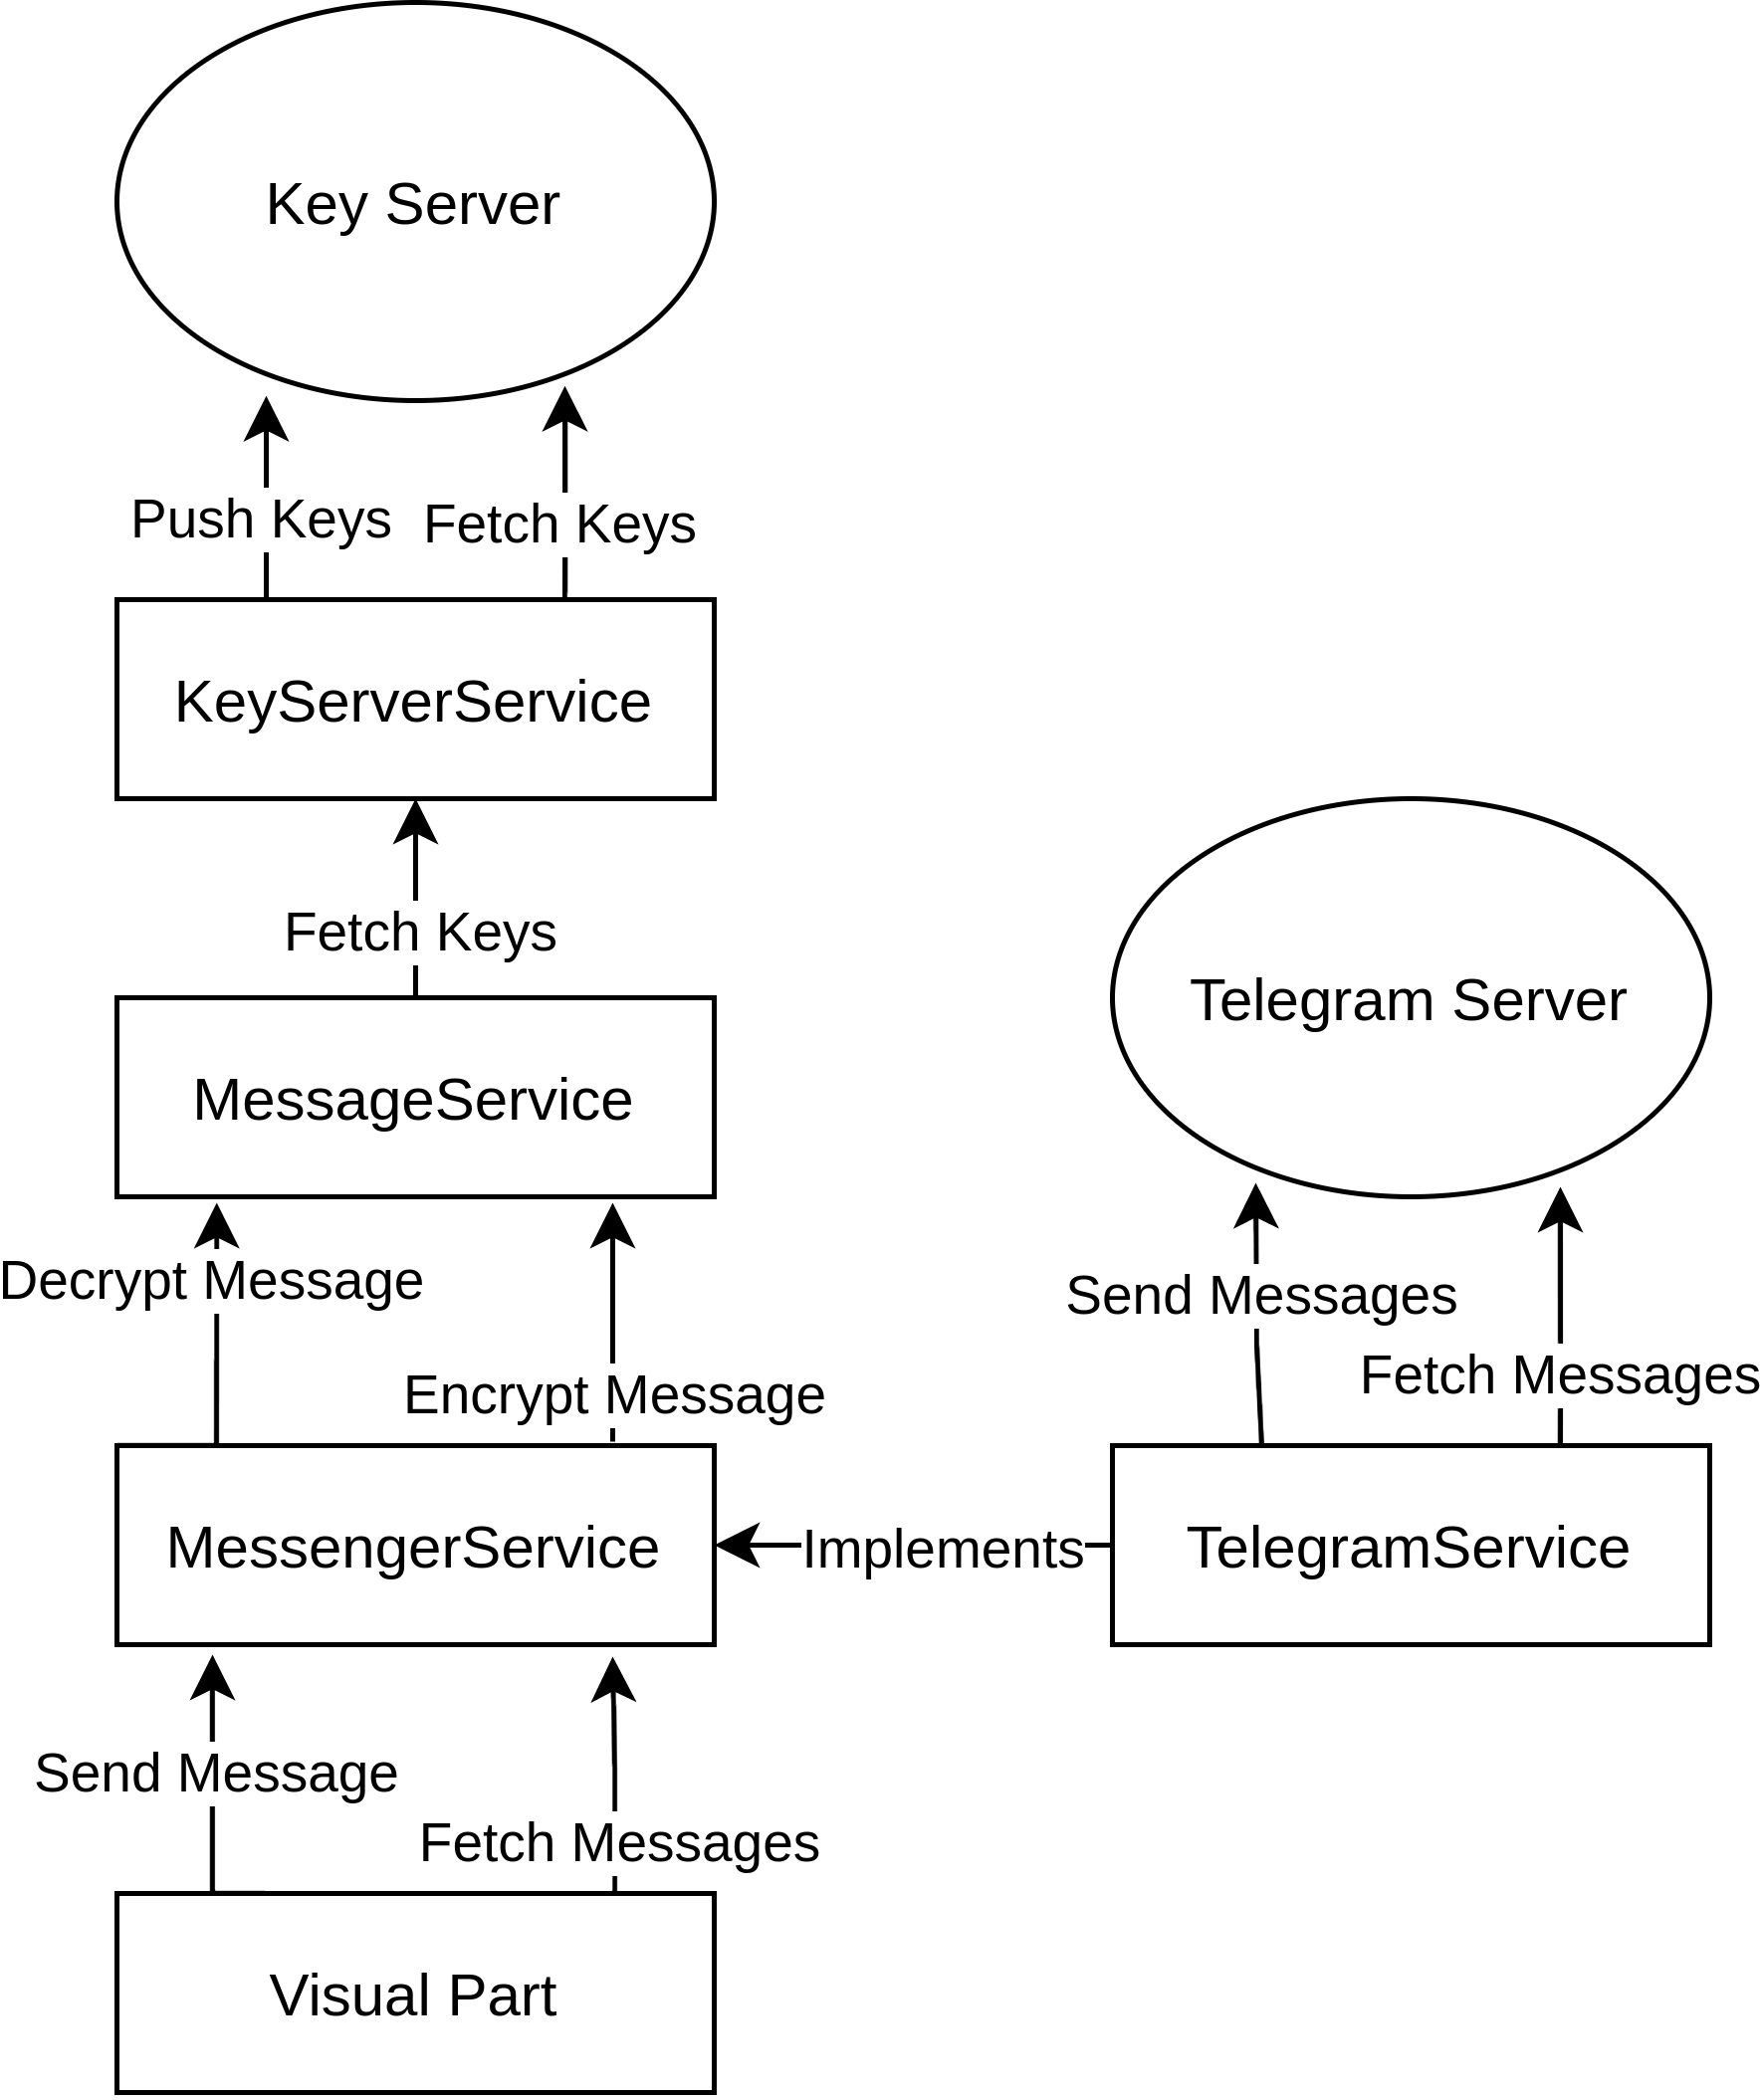
\includegraphics[width=\columnwidth]{figures/structure.png}
    \caption{Key Server Setup}
    \label{fig:structure}
\end{figure}




\section{Peer to Peer}
To encrypt a single message, a static symmetric key is used, that is known to both peers. The message is encrypted with the \emph{XSalsa20} algorithm, as used by Threema \cite{Threema}. The key is acquired through a Diffie-Hellman key exchange, also as in the Threema protocol, see Fig \ref{fig:peer_encryption}.

\begin{figure}[h!]
    \centering
    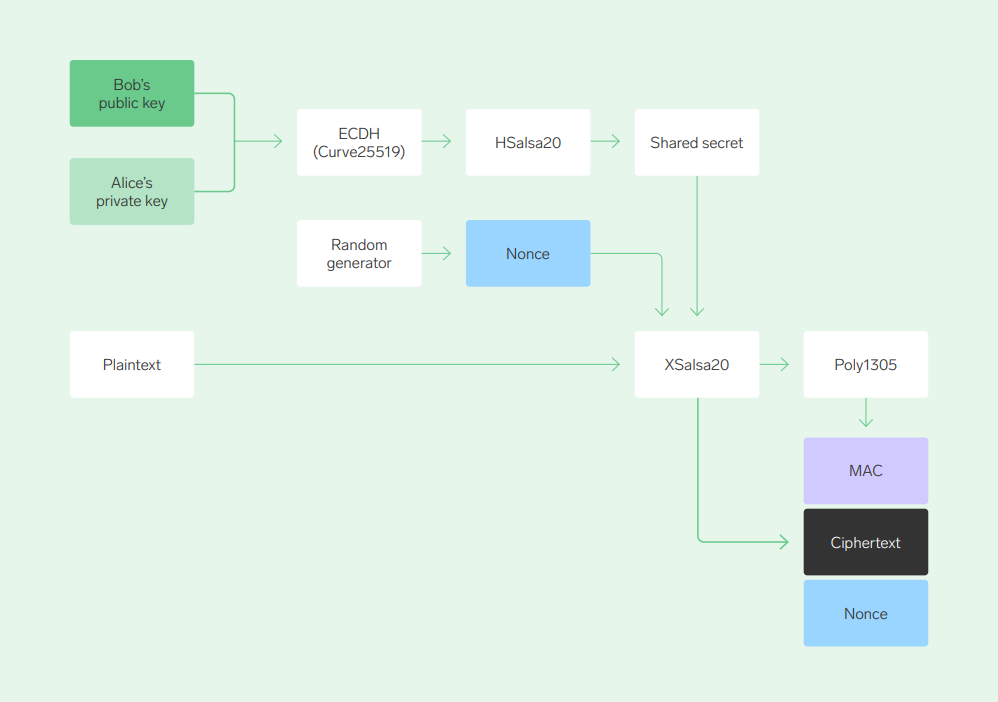
\includegraphics[width=\columnwidth]{figures/threema.png}
    \caption{The Peer to Peer encryption of Threema, from \cite{Threema}}
    \label{fig:peer_encryption}
\end{figure}

\subsection{Forward Secrecy}
\label{sec:forward_secrecy}

Currently, the most popular messengers have different approaches concerning forward secrecy. Signal and WhatsApp (which uses the Signal protocol), have a very sophisticated and utterly clever system, where after every message round trip, the symmetric encryption key is changed in a way, that if this specific version of the key is leaked, only the messages from the current round trip can be decrypted, but not past nor future messages. This is achieved by recursively hashing the key after every round trip (Ratching), and combining it with a new Diffie-Hellman key exchange after every round \cite{DoubleRatchet}.

In their device bound secret chats, Telegram does a re-keying after each 100 messages, and Threema refrains from implementing forward secrecy at all \cite{Threema}.

For the presented protocol, however, forward secrecy is not possible by design. Because a newly added device must be able to decrypt all previously sent messages in the cloud, forward secrecy cannot be achieved, because by definition in a forward secure system, a message should no longer be decryptable after it was sent and received once.

\subsection{Key Exchange}

For a Diffie-Hellman key exchange, two parties execute a synchronous protocol. But since in the context of mobile messaging this is not feasible, the protocol has to be made asynchronously. The proposed way is taken from Threema \cite{Threema}, but Signal's implementation is very close as well. First, both parties publish their public key part on an openly accessible server, here the key server is used. If party A wants to negotiate a key, it fetches the public key part of party B from the server, constructs the shared secret, and can already send the first messages. As soon as party B gets online, it can fetch party A's public key and also construct the same shared secret. The newly constructed symmetric keys are then saved on the key server. They could also easily be recreated each time a new device is added, but this way, as soon as the symmetric key was negotiated, user A is independent of user B. Even if user B deletes its account, user A can still decrypt the old messages.

\section{Groups}

Group chats are a bit more complex than peer to peer chats. Therefore, the existing messengers have different approaches to implement them.

\subsection{Signal/Threema}

Threema uses \emph{client side fan out}, a straight forward approach, where a group member sends group messages directly through peer to peer chats to the corresponding group members. The messages are tagged with the group ID. This approach is very easy, but it does not scale well, especially if the messages should be saved in the cloud. The used space per message is $\mathcal{O}(n)$, where $n$ are the number of group members \cite{Threema}. Because of this, for messages containing media, another approach was chosen, where the media is encrypted with a single symmetric key, which is distributed like a normal text message in the group. The media file is then stored on the Threema server until everybody has fetched it, or a timeout is reached.
In a blog post from 2014 Signal states that their group encryption also implements client side fan out, as Threema does \cite{SignalGroupsOld}. However, they use a more sophisticated system to manage group metadata, such that no information is leaked to the server \cite{SignalGroupsNew}.

\subsection{Whatsapp}

In their white paper, WhatsApp describes a \emph{server side fan out} system, where a group member first generates a random symmetric key, and sends it in a normal peer to peer chat to the other group members. The following messages are then encrypted with the symmetric key and sent to the server, which forwards it to each group member \cite{Whatsapp}. Key ratcheting is still possible with this approach. However, the new Diffie-Hellman key exchanges after each round trip are no longer possible, since there are more than two parties involved. Additionally, the messages are signed with an asymmetric key, to provide authenticity. It has to be mentioned, even though WhatsApp generally state that they use the Signal protocol for encryption, it is only used for peer to peer chats and calls, but not for group chats \cite{Newbedev}.

\subsection{Proposition}
On the base of the above protocols, a new one was proposed, which is optimized for the use as an overlay to a cloud-based messenger.

\subsubsection{Client Side Fan Out}
\label{sec:server_side_fan_out}

One approach would be to encrypt each message separately, and send them either over the classic peer to peer channel, with the group ID as a tag, or concatenate all encrypted version of the same message and send them as one large message in the group chat. The first option was discarded because it would mix the peer to peer chats with the group chats, which would add unnecessary complexity to the protocol. The second approach was also discarded, because it scales badly. Since text messages are relatively small, it would not be impossible, but it is also not very clean.

However, with both approaches, no additional measures are needed to handle the joining or leaving of group members. Since the group constellation is always known by the Telegram servers anyway, members could just encrypt their messages only for the current members of the group. It only leaves room for a relative harmless attack. A group member could just encrypt its message for everyone except one or more group members, and like this exclude them from the conversation. This however would be easily detectable by the affected members, and they could complain in the group chat. 

\subsubsection{Server Side Fan Out}

Another approach would be to use a single symmetric key for the group chat that is shared among all members. Like this, if a member wants to send a message, it would encrypt it only once, and send this message in the group chat.

With this approach, two problems arise. First, the symmetric key must be distributed among the members, and secondly, the key must be changed if the group constellation changes.

To solve the first problem, two solutions are proposed. The first one would be to encrypt a key with each peer to peer symmetric key, and send all encrypted keys concatenated into the group chat as one single Telegram message. This solution was discarded, because it would violate the separation of messages in the Telegram cloud and keys on the key server. The second and finally chosen solution, is to publish the set of individually encrypted keys on the key server. The key server holds a list for each group, where anyone who can authenticate itself, can append a new set of encrypted keys, together with the user ID of the poster. Since the server has no access to Telegrams group structure, it cannot check who is in which group. Therefore, it is the client's obligation to check if the latest key was really added by a group member. If not, it just fetches the second-latest key.

The problem of key renegotiation on joining or leaving was not completely solved yet due to time constraints, but it is discussed in detail in the chapter Future Work \ref{sec:future_work}.


\chapter{Implementation}




\section{Keyserver}

The key server is implemented in TypeScript and runs on Node.js. This has the advantage that the same language is used as for the app, and therefore the same libraries can be used in some cases. It is reachable under the domain \texttt{athena.eth-lerngruppe.ch}. The TypeScript framework used for the server is Express \cite{Express}. In this section, the most important concepts are described. A detailed API description can be found on  \href{https://gitlab.ethz.ch/disco-students/fs21/zarron_encrypted_chat/-/blob/1.0/Keyserver/API.md}{GitLab}.

\subsection{Keys}

\label{sec:keys}

Since many different keys are used in the protocol, first a short overview is presented, where the name, the purpose, the used algorithm of each key and its storage location is specified. Variables containing only the public part of a key are prepended by a \texttt{public\_} prefix. Variables containing the whole key, including the private part, are tagged with a \texttt{private\_} prefix.

\subsubsection{Authorization Key}

Name: \texttt{auth}

\noindent
Algorithm: ES512

\noindent
Usage: To authenticate to the key server

\noindent
Storage: Public part on the server, private part in the app

\subsubsection{Key Encryption Key}

Name: \texttt{sym}

\noindent
Algorithm: A256GCM

\noindent
Usage: To encrypt keys to store them on the key server

\noindent
Storage: In the app

\subsubsection{Group Key}

Name: \texttt{group}

\noindent
Algorithm: ECDH-ES, on curve P-521

\noindent
Usage: The public key is used by another group member to encrypt a new symmetric group key, which then can be decrypted by the owner of the private key.

\noindent
Storage: The public part publicly on the key server, the private part encrypted with \texttt{sym} on the key server.

\subsubsection{Peer Diffie-Hellman Key}

Name: \texttt{enc}

\noindent
Algorithm: ECDH, on curve 25519

\noindent
Usage: The public key is used by another user to agree on a symmetric key for peer to peer communication.

\noindent
Storage: The public part publicly on the key server, the private part encrypted with \texttt{sym} on the key server.

\subsection{Authentication}

To authenticate to the server, a token based system is used. In the following, the steps necessary to access a resource on the server are described.

\subsubsection{Account Creation}

On first use, an account has to be created. In the process, all keys specified in Section \ref{sec:keys} are created in the app. All keys except \texttt{private\_auth} and \texttt{sym} are sent to the server, see Lst. \ref{lst:new_account}. The server saves the received keys, and generates and returns a unique ID for the user.

\begin{listing}[h!]
\begin{minted}[frame=lines, linenos]{typescript}
{
    // public auth key of client
    "public_auth": "<key in pem format>",
    // public enc key of client
    "public_enc": "<key in base64>",
    // private encryption key of client, encrypted with auth
    "private_enc": "<key encrypted, in base64>",
    // used for symmetric group key encryption
    "public_group": "<key in JWK flattened format>",
    // used for symmetric group key decryption
    "private_group": "<key encrypted, JWE flattened format>" 
}
\end{minted}
\caption{JSON object sent to the key server on account generation}
\label{lst:new_account}
\end{listing}

\subsubsection{Token Aquistion}

All requests to the server, except for the account creation and the token acquisition requests, need to be authenticated. This is achieved by sending a JSON Web Token (JWT) with each request. To acquire this token, a user must complete a challenge, given by the server. The client first requests a nonce from the server, and creates a JSON Web Signature (JWS) object, that contains its ID and the nonce received previously by the server. This JWS is signed with the users \texttt{auth} key and sent to the server.

The server checks if the signature is valid for the \texttt{public\_auth} key saved for the ID of the sender. If the signature is valid, the server issues a JWT, containing the ID of the user and the expiration date, signed with the servers private \texttt{ed25519} key. Tokens are valid for two hours.

\subsubsection{Token Check}

Each time a user performs a request that has to be authenticated, a token must be added. The token is sent in the \texttt{authorization} header field, with the syntax \texttt{Bearer: <token>}. The server checks the validity of the signature, and if the token is not expired.

\subsection{Data Structure}

In the current state of the project, the user data is stored in two simple JSON files, \texttt{users.json} and \texttt{groups.json}. This makes it easier to debug. For scalability, a switch to a real database would be appropriate. Requests are handled sequentially without threading, to prevent race conditions.

\subsubsection{Users}

The \texttt{users.json} file consists of a list of user objects, specified in Lst. \ref{lst:users}. The user type contains a unique user ID, the keys transmitted during the account generation, optional IDs for Telegram or Facebook (which was not implemented, but would be in the next version) and an array of sessions, that contains the keys for peer to peer communications. The session keys are encrypted with the \texttt{sym} key.

There are specific requests to populate the \texttt{telegram} and \texttt{facebook} fields. They are called as soon as the users links an underlying messenger to its account.

The session keys are explained in more detail in Section \ref{sec:p2p_implementation}.


\begin{listing}[h!]
\begin{minted}[frame=lines, linenos]{typescript}
type Session = {
    "peer": string,
    "symmetric": string
}

type User = {
    "uuid": string,
    "public_auth": string,
    "public_enc": string,
    "private_enc": string,
    "public_group": string,
    "private_group": string,
    "sessions": Session[],
    "telegram"?: string,
    "facebook"?: string
};
\end{minted}
\caption{User objects, saved in \texttt{users.json}}
\label{lst:users}
\end{listing}

\subsubsection{Groups}
\label{sec:group_keys}

The \texttt{groups.json} contains an entry for each group, that specifies its ID, and the platform the group was created in (e.g. Telegram). This entry also contains a list of \texttt{GroupPosts}, as described in Lst. \ref{lst:groups}. A group post is created each time a new symmetric key is generated for this group. The symmetric key is then encrypted for each group member, and the resulting set is saved in the \texttt{group} field of the \texttt{GroupPost}. This process is explained in more detail in Section \ref{sec:groups_implementation}.

\begin{listing}[h!]
\begin{minted}[frame=lines, linenos]{typescript}
type GroupPost = {
    "from": string,
    "date": string
    "keys": GroupKey[] // entry for each group member
}

type GroupKey = {
    "uuid": string,
    "key": string // encrypted with user uuid's public_group key
}
\end{minted}
\caption{Group objects, saved in \texttt{groups.json}}
\label{lst:groups}
\end{listing}

\section{App}

The app was implemented with Ionic, using the Angular and Cordova framework \cite{Ionic}. It is a framework that allows the developer to compile a website to an app. Therefore, it is easy to develop cross-platform apps. The frameworks therefore use HTML and CSS for the visual part, and TypeScript for the logical part of the app.

\subsection{Structure}

The app is structured in three layers. The first layer, which is represented by the \texttt{KeyServerService}, handles the communication with the key server, and provides an interface to access the various keys. The second layer is represented by the \texttt{MessageService}, that provides an interface to encrypt messages. It uses the \texttt{KeyServerService} to get access to keys. The third layer handles communication with the APIs of the underlying cloud messengers. It provides an abstract base class (\texttt{MessengerService}), from which classes that implement the communication to specific messengers can inherit. Finally, there is also a visual part, that displays the messages received from the \texttt{MessengerService}. The structure is shown in Fig. \ref{fig:layers}.

\begin{figure}[h!]
    \centering
    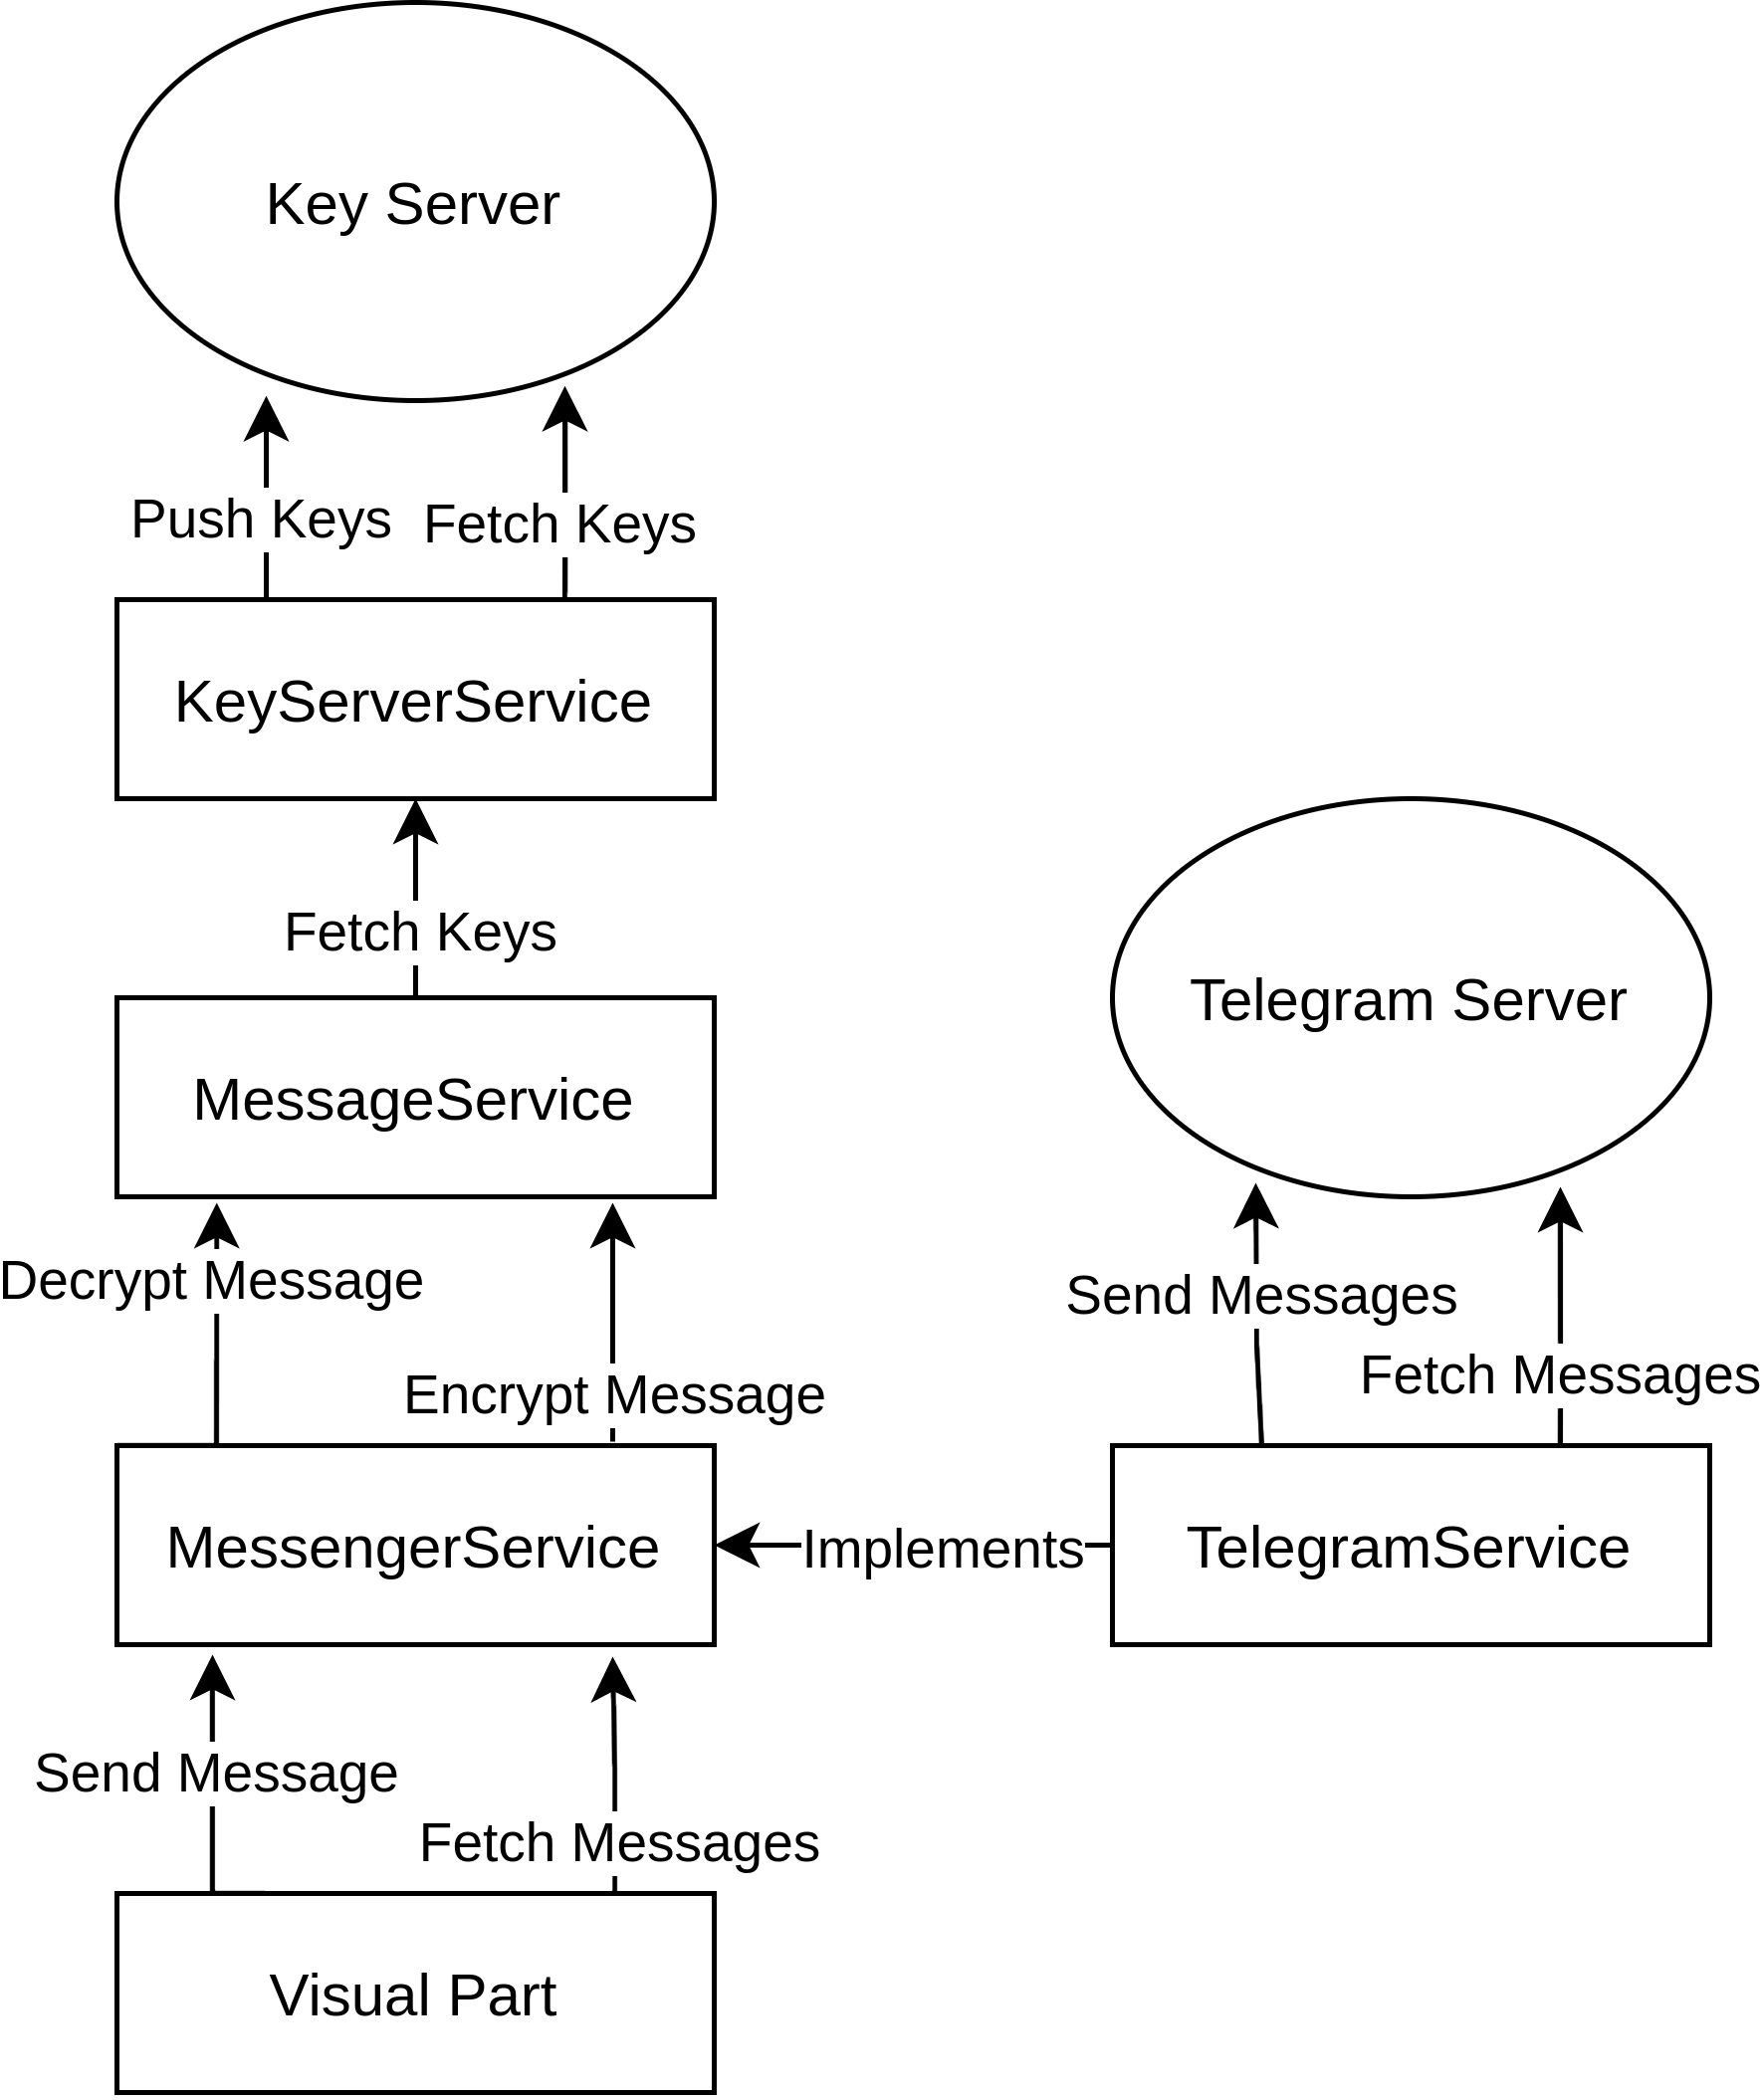
\includegraphics[width=0.8\columnwidth]{figures/layers.png}
    \caption{App Structure}
    \label{fig:layers}
\end{figure}


\subsection{Peer to Peer}
\label{sec:p2p_implementation}

Peer to peer messages are encrypted with a symmetric key, that is acquired through a Diffie-Hellman key agreement. This is implemented using the \texttt{TweetNaCl} library, a TypeScript implementation of the library Threema uses for its peer to peer chats \cite{Threema, TweetNaCl}. The library handles both key agreement and symmetric encryption.

The symmetric keys are acquired in the following way: First, it is checked if a key is already cached in the app, if not, the key server is checked for a symmetric key for this peer. If it is still no successful, the key server is queried for the \texttt{public\_enc} key of the peer. If it is present, a symmetric key is generated, using the \texttt{public\_enc} key of the peer and the \texttt{private\_enc} key of the user in question. The resulting symmetric key is then pushed to the key server. If the \texttt{public\_enc} key of the peer was not present on the server, it means that this peer does not use Athena yet, and the communication is continued in an unencrypted way.

If in the future more than one underlying cloud messenger can be linked to the app (e.g. Telegram and Facebook) and user A and user B both linked their Telegram and Facebook accounts to their Athena account, they would use the same symmetric key for peer to peer communication on both platforms. This comes from the decision that the \texttt{enc} key that is used to do Diffie-Hellman key agreements is unique per Athena account. It does however not pose a threat, since from a cryptographic view point, it is only a UI specific difference in which chat window the messages are shown, either Telegram or Facebook. In essence, it is only relevant that the messages are exchanged by user A and B.

\subsection{Groups}
\label{sec:groups_implementation}

Group messages are encrypted using a symmetric key, that is generated by one group member, and distributed to the others via the key server. For the message encryption, also the \texttt{TweetNaCl} library is used. In the current state of the app, only static groups are possible, which means that the constellation of members does not change. A system to modify group constellation is proposed in Section \ref{sec:group_member_changes}.



To acquire the symmetric key, first the apps cache is checked. If unsuccessful, the key server is queried. If the server does not contain a valid symmetric key for this group, a new one is created and posted in the following way:

The app first generates a random symmetric key. To make it accessible to all members of the group, but only to them, the key has to be encrypted and posted to the key server. Since the group members do not possess a shared key yet, the key has to be encrypted for each member individually. To achieve this, the \texttt{public\_group} key of each member is used. This results in a list of \texttt{GroupKey} objects, see Listing \ref{lst:groups}. This list is then posted to the key server. In the server, this data structure is called a \texttt{GroupPost}. However, if the key server would just provide a single slot for such a \texttt{GroupPost} per group, a malicious third party could just send random garbage to the server and fill this slot. This is possible, because the key server cannot know who is in which group, because it does not have access to the database of the underlying cloud messengers. Therefore, the key server cannot distinguish between a real group member and a user that is just pretending to be a member. To solve this issue, the key server maintains a list of \texttt{GroupPost} per group.

Users will always fetch the latest \texttt{GroupPost} first. Since the \texttt{GroupPost} object contains a field with the user ID of the poster, which is set by the key server, the users can easily detect if the \texttt{GroupPost} was posted by a user that is not a member of the group in question. If the post was from a malicious user, users can go through the list of \texttt{GroupPosts} chronologically until a valid post is found.

If a valid post was found, the user can go through the list of \texttt{GroupKeys}, until the entry for the user in question was found. The user can then decrypt the symmetric group key with its \texttt{private\_group} key.



\subsection{Visual Part}

In a chat, encrypted messages are displayed in blue, with a lock icon on the side. Unencrypted messages can still be read, but they are greyed out, see Figure \ref{fig:screenshots}. If an official client is used in parallel, encrypted messages are just displayed in their base64 encoded form, see Figure \ref{fig:chat_plain}. Also, a list of chats is implemented, with their latest message encrypted and displayed, see Figure \ref{fig:chats}.

\begin{figure}[h]
\begin{subfigure}{.5\textwidth}
  \centering
  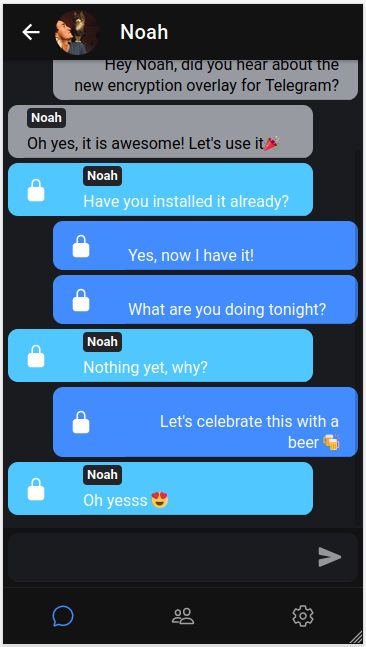
\includegraphics[width=.8\linewidth]{figures/chat_martin.png}
  \caption{Martin's Phone}
  \label{fig:chat_martin}
\end{subfigure}%
\begin{subfigure}{.5\textwidth}
  \centering
  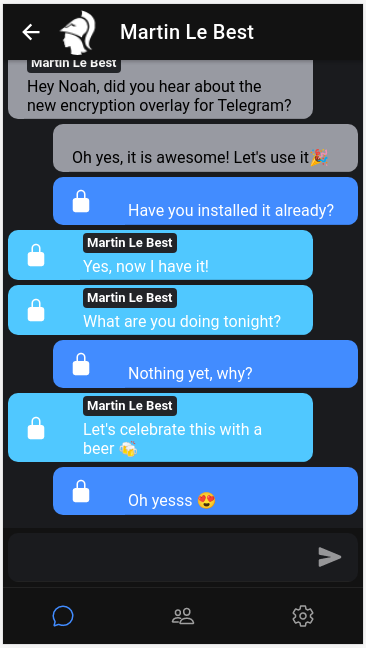
\includegraphics[width=.8\linewidth]{figures/chat_noah.png}
  \caption{Noah's Phone}
  \label{fig:chat_noah}
\end{subfigure}
\begin{subfigure}{.5\textwidth}
  \centering
  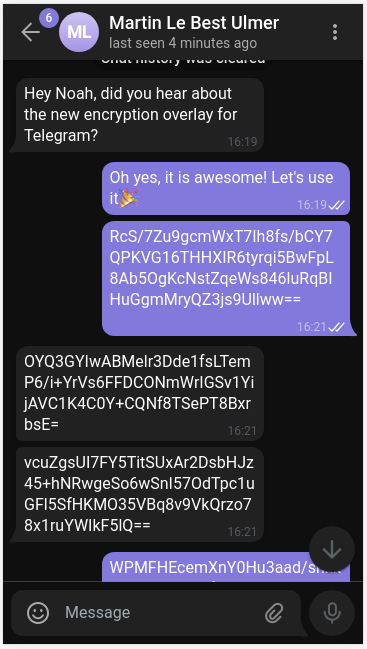
\includegraphics[width=.8\linewidth]{figures/chat_plain.png}
  \caption{Official Client}
  \label{fig:chat_plain}
\end{subfigure}%
\begin{subfigure}{.5\textwidth}
  \centering
  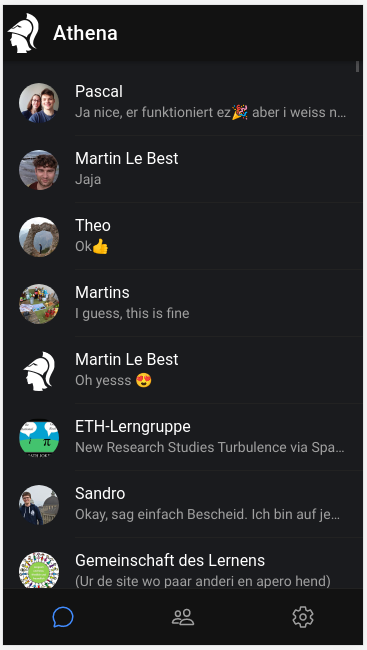
\includegraphics[width=.8\linewidth]{figures/chats.png}
  \caption{Chat List}
  \label{fig:chats}
\end{subfigure}
\caption{Screenshots}
\label{fig:screenshots}
\end{figure}


\chapter{Future Work}
\label{sec:future_work}

\section{Generic Additions}

Clearly, in the scope of one semester it is not possible to design a messenger client whose UI can compete with the existing messengers, that are developed by a whole team over years. Therefore, there could be a lot of time invested to improve the clients UI and add additional features, such as stickers, voice messages and so on.

Additionally, more underlying messengers could be added. Facebook would be a good option, because there already exist unofficial APIs.

Furthermore, the login system could be improved, currently it only consists of a pop-up that asks for credentials that have to be entered by hand.

\section{In Platform Authentication}

In the current implementation, anybody can make an Athena account in the app, which is fine. However, anybody can also link an arbitrary Telegram account to its account, just by posting its Telegram ID to the key server, which is publically known. Like this, a malicious user can relatively easy impersonate another user. This problem could be solved by implementing a Telegram bot (or a service account in Facebook). If a user wants to link its Telegram account to the server, it could authenticate itself to the server with its unique user ID, and request a nonce. This nonce has to be sent to this Telegram bot by the user in question. The bot can then forward the sender Telegram ID together with the nonce to the key server.

\section{Group Modifications}

In the current implementation, groups are static, which means that no members can be added or removed. Also, there is no system for group members to accuse malicious members.

\subsection{Malicious Members}

Right now, it is possible for anybody to publish a new \texttt{GroupPost} to the key server, containing a new symmetric key. If the user who published the \texttt{GroupPost} was not in the group, it is just ignored. However, it is also possible for a group member to be malicious. While encrypting the symmetric key for each member, a malicious user could just encrypt random garbage for a specific member. This member would then de facto be excluded from the group, until a new key would be published. However, the affected user can never be completely sure if the poster of the \texttt{GroupPost} was really malicious, or if everybody else in the group is just using the official unencrypted Telegram client at the moment, and therefore these unencrypted messages cannot be decrypted anyway.

To resolve this uncertainty, an additional check could be implemented. To the \texttt{GroupPost} an additional field could be added. This would contain a well known text, for example "How do you turn this on?", that is encrypted with the symmetric key, promoted in this \texttt{GroupPost}. After decrypting their version of the symmetric key, the group members could check if they can decrypt the well known text with their version of the symmetric key. If not, they know for sure that the user who posted the \texttt{GroupPost} was malicious. In this case, the user could just post a new \texttt{GroupPost} with a real key. Additionally, a system could be implemented to prove to the other group members that the user in question is malicious. But for this, there is no solution sketch yet.

\subsection{Member Changes}
\label{sec:group_member_changes}
For a fully functional messenger overlay, it should be possible to add or remove members to the group. This is no yet fully supported in the current implementation. If the group constellation changes, a new key has to be posted. To make messages encrypted with an old key still decryptable, it would make sense to assign an ID to each \texttt{GroupPost}, and append this ID to each message that is encrypted with the symmetric key associated with this ID. Like this, posting new keys has no negative effects, except for an increased storage use on the server. Therefore, a member that newly joined the group could just post a new key. If a member leaves the group, the next user that wants to send a message would just post a new \texttt{GroupPost} first, to make it impossible for the former member to decrypt newly sent messages.

\section{Efficiency}

In the current implementation, only the most crucial optimizations were applied. There is still much room for optimizations.

\subsection{Message Cacheing}

Currently, each time the app is loaded, or a chat is opened, all contacts, messages and profile pictures are fetched again from the server. In a future version, this data could be cached on the disk, such that it would also be available for offline use. It could also be used to bypass a blank loading screen if the device is online.

Furthermore, a messenger needs a system to periodically check for new messages to display them. Currently, all messages are refetched every second from the messaging server. Telegram would even offer a system to only query changed data, but for compatibility reasons with future messengers, the brute force method is chosen. But there would also be room for a better solution.

\subsection{Key Chacheing}

In the current implementation, peer to peer symmetric keys and group symmetric keys are fetched once at the start of the app, and then cached for further use in RAM. They could also be cached on disk for faster initial loading times.

\chapter{Conclusion}

The goal of this work was to design and implement a client that adds end-to-end encryption to a generic cloud-based messenger. A large part of the work consisted in analyzing the existing messengers and cherry-picking their best solutions.

The final version of the app reaches all its desired properties, however, there is still room for many additional features. What could not be achieved, is the addition of forward secrecy to the used protocol. This turned out to be incompatible with the cloud nature of the underlying messengers. Also, the underlying messengers are still able to collect metadata, since even tough they cannot decrypt messages anymore, they can still observe who is communicating with whom. 

Finally, the presented client provides a good tradeoff between convenience and security. For a typical user, the security can be considered sufficient. However, people that are reliant on a completely save messenger should switch to Signal. It is by far the best messenger in terms of privacy and security. 

% This displays the bibliography for all cited external documents. All references have to be defined in the file references.bib and can then be cited from within this document.
\bibliographystyle{IEEEtran}
\bibliography{references}

% This creates an appendix chapter, comment if not needed.
\appendix
\chapter{Code}

The code for the app and the key server are available on GitLab:

\url{https://gitlab.ethz.ch/disco-students/fs21/zarron_encrypted_chat/-/tree/1.0/}

\end{document}